\documentclass[12pt,a4,oneside,usenames,dvipsnames]{book}
  \usepackage{polyglossia}
  \usepackage{fontspec}
  \setmainlanguage{english}
  \setotherlanguage{greek}
  \setmainfont{Redaction}
  \usepackage{unicode-math}
  %\setmathfont{Latin Modern Math}
  \setmathfont{TeX Gyre Pagella Math}
  \setmonofont[Scale=1.1]{CMU Typewriter Text}
  \newfontfamily\pixelfont{Redaction35-Regular}
  \newfontfamily\fira[Scale=0.90]{Fira Sans}
  \newfontfamily\thumbfont[Scale=0.9]{Redaction35-Bold}
  \newfontfamily\pixeltitle[Scale=3.5]{Redaction35-Bold}
  \newfontfamily\reduxtitle[Scale=3.5]{Redaction-Bold}
  \newfontfamily\cm{CMU Serif}
  \usepackage{microtype}
  \usepackage{graphicx}
  \usepackage{dot2texi}
  \usepackage[breaklinks=true]{hyperref}
\hypersetup{
    unicode,
    verbose=false,
    pdfpagelayout=TwoColumnRight,
    bookmarksopen,
    colorlinks,
    citecolor=black,
    filecolor=black,
    linkcolor=black,
    urlcolor=black
}
\usepackage[nobiblatex]{xurl}
\usepackage{makeidx}
\makeindex
\usepackage[totoc]{idxlayout}
  \usepackage{microtype}
  \usepackage{marginnote}
  \usepackage[noclrdblpg]{colophon}
  \usepackage{bookmark}
  \usepackage{amsmath}
  \usepackage{float}
  \usepackage{skeldoc}
  \floatplacement{figure}{H}
  \usepackage{tikz}
  \usepackage{svg}
  \usepackage{calc} % for inkscape pdf tex
  \usepackage{attachfile2}
%\usepackage[showframe,marginparwidth=3cm,twoside=true]{geometry}
\usepackage[marginparwidth=3cm,twoside=true,a4paper]{geometry}
  \usepackage{metalogo}
  \usepackage{csquotes}
  \usepackage[compact,nostruts,medium]{titlesec}
  %\titlespacing*{\chapter}{0pt}{0pt}{0pt}
  \newcommand\makeskelfig{%
  \begin{figure}
  {\centering%
  \skelfig[width=0.4\textwidth]{2\baselineskip}%
  \skelcaption[width=0.2\textwidth,lines=1]{}}
  \end{figure}}
  \usepackage{setspace}
  \definecolor{blackoutline}{RGB}{14,14,14}
  \definecolor{bgcolor}{rgb}{0.95,0.95,0.95}
  \definecolor{red}{rgb}{1,0,0}
  \definecolor{gray}{RGB}{24,24,24}
   \definecolor{thered}    {rgb} {0.65,0.04,0.07}
 \definecolor{thegreen}  {rgb} {0.06,0.44,0.08}
 \definecolor{theblue}   {rgb} {0.02,0.04,0.48}
 \definecolor{sectioning}{gray}{0.44}
 \definecolor{thegrey}   {gray}{0.5}
 \definecolor{theframe}  {gray}{0.75}
 \definecolor{theshade}  {gray}{0.94}
 \definecolor{thepeach}  {RGB}{246,232,220}
 \definecolor{punchbg}{RGB}{250, 230, 180}
 \definecolor{punchframe}{RGB}{240, 220, 170}
\usepackage[cache=false,outputdir=build]{minted}
\setminted[rust]{labelposition=bottomline,bgcolor=thepeach,rulecolor=punchframe,fontsize=\scriptsize,baselinestretch=0.5,frame=leftline,breaklines=true,breakanywhere=true}
\setminted[c]{bgcolor=theshade,fontsize=\scriptsize,baselinestretch=0.5,frame=leftline,breaklines=true,breakanywhere=true}
%\setminted[tex]{breaklines=true,linenos=true,bgcolor=theshade,frame=single,framesep=5pt,rulecolor=theframe}
%\setminted[shell]{breaklines=true,linenos=true,bgcolor=theshade,frame=single,framesep=5pt,rulecolor=theframe}
%\definecolor{bg}{rgb}{0.95,0.95,0.95}
\usepackage{xspace}
\usepackage{xparse}
\usepackage{contour}
\usepackage[normalem]{ulem}
\usepackage{minted}
\usemintedstyle{bw}

\ExplSyntaxOn
\NewDocumentCommand{\TitleOutline}{m}
 {
  \seq_set_split:Nnn \l_tmpa_seq { ~ } { #1 }
  \seq_map_inline:Nn \l_tmpa_seq { \contour{blackoutline}{##1} ~ } \unskip
 }
\ExplSyntaxOff

\renewcommand{\ULdepth}{1.8pt}
\contourlength{0.8pt}

\makeatletter
\renewcommand\@dotsep{200}
\renewcommand{\l@chapter}{\@dottedtocline{0}{0pt}{2.6em}}
\renewcommand{\l@section}{\@dottedtocline{1}{1.5em}{2.6em}}
\renewcommand{\l@subsection}{\@dottedtocline{2}{4.0em}{3.6em}}
\renewcommand{\l@subsubsection}{\@dottedtocline{3}{7.4em}{4.5em}}
\makeatother

\newcommand\bitmap{{\pixelfont{}bitmap}}
\newcommand\bitmaps{{\pixelfont{}bitmaps}}
\newcommand\pixel{{\pixelfont{}pixel}}
\newcommand\pixels{{\pixelfont{}pixels}}
\newcommand\Rust{{\fira{}\textbf{Rust}}}

\newcommand\colorunderline[1]{\bgroup\markoverwith{\textcolor{#1}{\rule[-0.5ex]{2pt}{0.8pt}}}\ULon}
\newcommand{\myuline}[2]{%
  \colorunderline{#1}{\phantom{#2}}%
  \llap{\contour{white}{#2}}%
}
\DeclareRobustCommand{\myurl}[2]{%
  \href{#1}{\myuline{blue}{#2}}%
}

\newcommand{\attachsource}[1]{%
\marginnote{\scriptsize{}%
\texttt{\tiny{}#1}:\\
\attachfile[icon=Paperclip]{#1}\hfill\\
This code file is a PDF attachment}%
}%
\newcommand\titletext{A {\pixeltitle{}Bitmapper}'s Companion}
\newcommand\covertitletext{\TitleOutline{A {\pixeltitle{}Bitmapper}'s Companion}}
\title{\titletext{}}
\newcommand\subtitle{an introduction to basic \bitmap{} mathematics and algorithms with code samples in \Rust{}}
\newcommand\coversubtitle{\TitleOutline{an introduction to basic \bitmap{} mathematics and algorithms with code samples in \Rust{}}}
\newcommand\biblatex{\texttt{biblatex}\xspace}%
\hypersetup{
  pdftitle={\titletext{}},
  pdfauthor={epilys},
  pdfsubject={programming},
}
\usepackage{wallpaper}

\newsavebox{\mintedbox}

\usepackage[thumblink=line,height=50pt,minheight={50pt},width=50pt,distance={2mm},topthumbmargin={5cm},bottomthumbmargin={2pt},eventxtindent={0pt},oddtxtexdent={2pt},evenmarkindent={0pt},oddmarkexdent={0pt},evenprintvoffset={0pt},nophantomsection=false,ignorehoffset=true,ignorevoffset=true,final=true,hidethumbs=false,verbose=true]{thumbs}
 \definecolor{DarkBg}  {rgb} {0.17,0.17,0.17}
 \definecolor{DarkFg}  {rgb} {0.90,0.90,0.90}
 \definecolor{LightBg} {rgb}{1.0,1.0,1.0}
\newcommand{\setbackgroundcolour}{\pagecolor{DarkBg}}
\newcommand{\settextcolour}{\color[rgb]{0.90,0.90,0.90}}
\newcommand{\invertbackgroundtext}{\setbackgroundcolour\settextcolour}
\newcommand{\revertbackgroundcolour}{\pagecolor{LightBg}}
\newcommand{\reverttextcolour}{\color[rgb]{0.19,0.19,0.19}}
\newcommand{\revertbackgroundtext}{\revertbackgroundcolour\reverttextcolour}

\newcommand\myaddthumb[2]{%
  %\addtitlethumb{#1}{\fcolorbox{red}{black}{\parbox[t][45pt]{45pt}{\noindent%
  \addtitlethumb{\hspace{5pt}#1}{%
    \parbox[t][43pt]{43pt}{\centering
    \vfill\noindent%
{\linespread{.7}\thumbfont{}#2\par\vfill}%
}%
}{white}{DarkBg}{pagesLTS.0}%
}%

\pagenumbering{arabic}

  \usepackage[textsize=tiny]{todonotes}
\begin{document}
\newgeometry{left=1cm,top=0.1cm,right=1cm,bottom=0.1cm}
\pdfbookmark{Title page}{title-page}%cover
\ThisLRCornerWallPaper{0.55}{Holbein_Skull2_inverted.png}
\setstretch{1.1}
\invertbackgroundtext
\addtolength{\parskip}{5pt}%
\newlength\drop
\thispagestyle{empty}
\begingroup% Harry Carter
\setlength{\drop}{0.1\textheight}
\vspace*{\drop}
\begin{flushleft}
  \textcolor{thegrey}{\rule{\textwidth}{1.6pt}}%
  \vspace{-0.9\baselineskip}
  \textcolor{sectioning}{\rule{\textwidth}{0.4pt}}\\[0.8\baselineskip]
  {\centering
  \contourlength{0.02em}
  \scalebox{2.0}{\parbox{0.5\textwidth}{\centering{\reduxtitle{}\covertitletext{}}}}\\
  \vspace{.8\baselineskip}
  \par
  \vspace{-0.4\baselineskip}
  }\textcolor{thegrey}{\rule{\textwidth}{1.6pt}}%
  \vspace{-0.9\baselineskip}
  \textcolor{sectioning}{\rule{\textwidth}{0.4pt}}\\[0.2\baselineskip]
  {\Large{}\TitleOutline{epilys}}\hfill{\small{}\TitleOutline{\today{}}}
  \vfill%
  \scalebox{1.5}{\parbox{0.28\textwidth}{\noindent%
  {\LARGE\raggedleft\coversubtitle{}\par}
  }}
  \vfill%
\end{flushleft}%
\endgroup
\clearpage{}
\restoregeometry
\revertbackgroundtext
\clearpage{}
.
\clearpage{}
\thumbsoverview{map}
\clearpage{}
\marginnote{
\includegraphics{xface.png}}[-1.3\baselineskip]\noindent{}Manos Pitsidianakis (epilys)\\
\myurl{https://nessuent.xyz}{https://\-nessuent.xyz}\\
\myurl{https://github.com/epilys}{https://github.com/epilys}\\
\myurl{epilys@nessuent.xyz}{epilys@nessuent.xyz}\\

\noindent{}All non-screenshot figures were generated by hand in Inkscape unless otherwise stated.

\noindent{}The skull in the cover is a transformed bitmap of the skull in the 1533 oil painting by Hans Holbein the Younger, \emph{The Ambassadors}, which features a floating distorted skull rendered in anamorphic perspective.

\noindent{}\emph{A Bitmapper’s Companion}, 2021\\
\noindent{}\textbf{Special Topics} $\blacktriangleright{}$ \textbf{Computer Graphics} $\blacktriangleright{}$ \textbf{Programming}\\
\noindent{}006.6'6--dc20
\vfill{}
\noindent{}Copyright © 2021 by Emmanouil Pitsidianakis

\noindent{}This work is licensed under the Creative Commons Attribution-NonCommercial-ShareAlike 3.0 Unported License. To view a copy of this license, visit\\\myurl{http://creativecommons.org/licenses/by-nc-sa/3.0/}{http\-:\-//\-creativecommons\-.\-org\-/\-licenses\-/\-by-nc-sa/3.0/} or send a letter to Creative Commons, PO Box 1866, Mountain View, CA 94042, USA.

\noindent{}The source code for this work is available under the GNU GENERAL PUBLIC LICENSE version 3 or later. You can view it, study it, modify it for your purposes as long as you respect the license if you choose to distribute your modifications.

\noindent{}The source code is available here

\noindent{}\myurl{https://github.com/epilys/bitmappers-companion}{https://github.com/epilys/bitmappers-companion}

\clearpage{}
\myaddthumb{Table Of Contents}{toc}
\pdfbookmark{\contentsname}{toc}
\ThisLRCornerWallPaper{0.6}{The-Ambassadors.png}
\tableofcontents
\ThisLRCornerWallPaper{0.4}{Holbein_Skull.png}
\clearpage{}
\myaddthumb{Introduction}{intro}
\part{Introduction}
\chapter{Data representation}
The data structures we're going to use is \emph{Point} and \emph{Image}. \emph{Image} represents a \bitmap{}, although we will use full RGB colors for our points therefore the size of a \pixel{} in memory will be \texttt{u8} instead of 1 bit.

We will work on the cartesian grid representing the framebuffer that will show us the \pixels{}. The \emph{origin} of this grid (i.e. the center) is at $(0,0)$.%
\begin{figure}%
\centering
\input{cartesian_grid.pdf_tex}
\end{figure}%
%
We will represent points as pairs of signed integers. When actually drawing them though, negative values and values outside the window's geometry will be ignored (clipped).
%
\attachsource{src/lib.rs}
%
\begin{minted}{rust}
pub type Point = (i64, i64);

pub const fn from_u8_rgb(r: u8, g: u8, b: u8) -> u32 {
    let (r, g, b) = (r as u32, g as u32, b as u32);
    (r << 16) | (g << 8) | b
}
pub const AZURE_BLUE: u32 = from_u8_rgb(0, 127, 255);
pub const RED: u32 = from_u8_rgb(157, 37, 10);
pub const WHITE: u32 = from_u8_rgb(255, 255, 255);
pub const BLACK: u32 = 0;

pub struct Image {
    pub bytes: Vec<u32>,
    pub width: usize,
    pub height: usize,
    pub x_offset: usize,
    pub y_offset: usize,
}

impl Image {
    pub fn new(width: usize, height: usize, x_offset: usize, y_offset: usize) -> Self;
    pub fn draw(&self, buffer: &mut Vec<u32>, fg: u32, bg: Option<u32>, window_width: usize);
    pub fn draw_outline(&mut self);
    pub fn clear(&mut self);
    pub fn plot(&mut self, x: i64, y: i64);
    pub fn get(&mut self, x: i64, y: i64) -> u32;
    pub fn plot_ellipse(
        &mut self,
        (xm, ym): (i64, i64),
        (a, b): (i64, i64),
        quadrants: [bool; 4],
        _wd: f64,
    );
    pub fn plot_line_width(&mut self, point_a: Point, point_b: Point, wd: f64);
    pub fn flood_fill(&mut self, mut x: i64, y: i64);
}
\end{minted}

\chapter{Displaying {\pixels{}} to your screen}
A way to display an \emph{Image} is to use the \texttt{minifb} crate which allows you to create a window and draw \pixels{} directly on it. Here's how you could set it up:
%
\attachsource{src/bin/introduction.rs}
%
%
\begin{minted}{rust}
use bitmappers_companion::*;
use minifb::{Key, Window, WindowOptions};

const WINDOW_WIDTH: usize = 400;
const WINDOW_HEIGHT: usize = 400;

fn main() {
    let mut buffer: Vec<u32> = vec![WHITE; WINDOW_WIDTH * WINDOW_HEIGHT];
    let mut window = Window::new(
        "Test - ESC to exit",
        WINDOW_WIDTH,
        WINDOW_HEIGHT,
        WindowOptions {
            title: true,
            //borderless: true,
            //resize: false,
            //transparency: true,
            ..WindowOptions::default()
        },
    )
    .unwrap();

    // Limit to max ~60 fps update rate
    window.limit_update_rate(Some(std::time::Duration::from_micros(16600)));

    let mut image = Image::new(50, 50, 150, 150);
    image.draw_outline();
    image.draw(&mut buffer, BLACK, None, WINDOW_WIDTH);

    while window.is_open()
         && !window.is_key_down(Key::Escape)
         && !window.is_key_down(Key::Q) {
        window
            .update_with_buffer(&buffer, WINDOW_WIDTH, WINDOW_HEIGHT)
            .unwrap();
        let millis = std::time::Duration::from_millis(100);
        std::thread::sleep(millis);
    }
}
\end{minted}

Running this will show you something like this:
% FIXME reduce window size and resulting screenshot size

\begin{figure}[H]
\centering
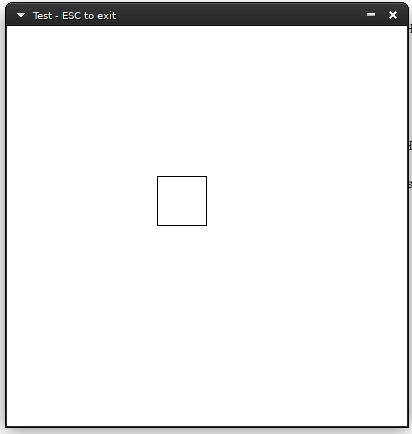
\includegraphics{figures/introduction.png}
\end{figure}

\chapter{Bits to byte \pixels{}}
Let's define a way to convert bit information to a byte vector:

\begin{minted}{rust}
pub fn bits_to_bytes(bits: &[u8], width: usize) -> Vec<u32> {
    let mut ret = Vec::with_capacity(bits.len() * 8);
    let mut current_row_count = 0;
    for byte in bits {
        for n in 0..8 {
            if byte.rotate_right(n) & 0x01 > 0 {
                ret.push(BLACK);
            } else {
                ret.push(WHITE);
            }
            current_row_count += 1;
            if current_row_count == width {
                current_row_count = 0;
                break;
            }
        }
    }
    ret
}
\end{minted}

\chapter{Loading \texttt{xbm} files in \Rust{}}

\emph{The end of this chapter includes a short \Rust{} program to automatically convert \texttt{xbm} files to equivalent \Rust{} code.}

\texttt{xbm} files are C source code files that contain the \pixel{} information for an image as macro definitions for the dimensions and a static \texttt{char} array for the \pixels{}, with each bit column representing a pixel. If the width dimension doesn't have 8 as a factor, the remaining bit columns are left blank/ignored.

They used to be a popular way to share user avatars in the old internet and are also good material for us to work with, since they are small and numerous. The following is such an image:

\begin{figure}[H]
\centering

\includegraphics{figures/news.png}
\end{figure}
%FIXME
Then, we can convert the \texttt{xbm} file from C to \Rust{} with the following transformations:

\begin{minted}{c}
#define news_width 48
#define news_height 48
static char news_bits[] = {
\end{minted}

to


\begin{minted}{rust}
const NEWS_WIDTH: usize = 48;
const NEWS_HEIGHT: usize = 48;
const NEWS_BITS: &[u8] = &[
\end{minted}

And replace the closing \texttt{\}} with \texttt{]}.

We can then include the new file in our source code:


\begin{minted}{rust}
include!("news.xbm.rs");
\end{minted}

load the image:

\begin{minted}{rust}
let mut image = Image::new(NEWS_WIDTH, NEWS_HEIGHT, 25, 25);
image.bytes = bits_to_bytes(NEWS_BITS, NEWS_WIDTH);
\end{minted}

and finally run it:

\begin{figure}[H]
\centering

\includegraphics{figures/intro-2.png}
\end{figure}

The following short program uses the \texttt{regex} crate to match on these simple rules and print the equivalent code in \texttt{stdout}. You can use it like so:

\begin{minted}{shell}
cargo run --bin xbmtors -- file.xbm > file.xbm.rs
\end{minted}
\attachsource{src/bin/xbmtors.rs}

\begin{minted}{rust}
use regex;
use regex::Regex;
use std::fs::File;
use std::io::prelude::*;

fn main() {
    let args = std::env::args().skip(1).collect::<Vec<String>>();
    if args.len() != 1 {
        println!("one argument expected, the xbm file path to convert.");
        return;
    }
    let mut file = match File::open(&args[0]) {
        Err(err) => panic!("couldn't open {}: {}", args[0], err),
        Ok(file) => file,
    };

    let mut s = String::new();
    if let Err(err) = file.read_to_string(&mut s) {
        panic!("couldn't read {}: {}", args[0], err);
    }

    let re = Regex::new(
        r"(?imx)
  ^\s*\x23\s*define\s+(?P<i>.+?)_width\s+(?P<w>\d\d*)$
  \s*
  ^\s*\x23\s*define\s+.+?_height\s+(?P<h>\d\d*)$
  \s*
  ^\s*static(\s+unsigned){0,1}\s+char\s+.+?_bits..\s*=\s*\{(?P<b>[^}]+)\};
",
    )
    .unwrap();

    let caps = re
        .captures(&s)
        .expect("Could not convert file, regex doesn't match :(");
    let ident = caps.name("i").unwrap().as_str().to_uppercase();
    let out = re.replace_all(&s, format!("const {i}_WIDTH: usize = $w;\nconst {i}_HEIGHT: usize = $h;\nconst {i}_BITS: &[u8] = &[$b];", i = &ident));
    println!("{}", out.trim());
}
\end{minted}
\clearpage{}
\myaddthumb{Points And Lines}{lines}
\part{Points And Lines}
\chapter{Distance between two points}

\begin{figure}
\centering
\input{fig1.pdf_tex}
\end{figure}

Given two points, $K$ and $L$, an elementary application of Pythagoras' Theorem gives the distance between them as

\begin{equation}
  r = \sqrt{(x_{L} - x_{K})^{2} +(y_{L} - y_{K})^{2}}
\end{equation}
which is simply coded:
\begin{minted}{rust}
pub fn distance_between_two_points(p_k: Point, p_l: Point) -> f64 {
    let (x_k, y_k) = p_k;
    let (x_l, y_l) = p_l;
    let xlk = x_l - x_k;
    let ylk = y_l - y_k;
    f64::sqrt((xlk*xlk + ylk*ylk) as f64)
}
\end{minted}
\chapter{Equations of a line}\label{ch:equations-lines}
There are several ways to describe a line mathematically. We'll list the convenient ones for drawing \pixels{}.

The equation that describes every possible line on a two dimensional grid is the \emph{implicit} form $ax+by=c, (a,b) \neq{} (0,0)$. We can generate equivalent equations by adding the equation to itself, i.e. $ax+by=c \equiv 2ax+2by=2c \equiv a'x+b'y=c', a'=2a, b'=2b, c'=2c$ as many times as we want. To "minimize" the constants $a,b,c$ we want to satisfy the relationship $a^{2}+b^{2}=1$, and thus can convert the equivalent equations into one representative equation by multiplying the two sides with $\frac{1}{\sqrt{a^2+b^2}}$; this is called the normalized equation. % TODO: why? add footnote: in the normalized form, a is the cosine of the angle the normal vector makes with the x axis, and b the cosine of the angle with the y axis. and c = - (dist of line to the origin)

The \emph{slope intercept form} describes any line that intercepts the $y$ axis at $b \in{} \mathbb{R}$ with a specific slope $a$:

$$y=ax+b$$

The \emph{parametric} form... % TODO

%% TODO: add conversion between forms

\section{Line through a point $P=(x_p,y_p)$ and a slope $m$}

$$y-y_p=m(x-x_p)$$

\section{Line through two points}
\begin{figure}
\centering
\input{line_through_points.pdf_tex}
\end{figure}
It seems sufficient, given the coordinates of two points $M, N$, to calculate $a, b$ and $c$ to form a line equation:

$$ax+by+c=0$$

If the two points are not the same, they necessarily form such a line. To get there, we start from expressing the line as parametric over $t$: at $t=0$ it's at point $M$ and at $t=1$ it's at point $N$:

$$c = c_M + (c_N - c_M)t, t\in R, c \in \{x, y\}$$
$$c = c_M, t\in R, c \in \{x, y\}$$

Substituting $t$ in one of the equations we get:

$$(y_M - y_N)x + (x_N-x_M)y+(x_{M}y_{N}-x_{N}y_{M})=0$$

Which is what we were after. We finish by normalising what we found with $\frac{1}{\sqrt{a^2+b^2}}$:
\begin{minted}{rust}
\end{minted}

\chapter{Distance from a point to a line}
\todo[inline]{Add code samples in \emph{Distance from a point to a line}}
\begin{figure}
\centering
\input{point_line_distance.pdf_tex}
\end{figure}

\section{Using the implicit equation form}
Let's find the distance from a given point $P$ and a given line $L$. Let $d$ be the distance between them. Bring $L$ to the implicit form $ax+by=c$.

$$d= \frac{|ax_p+by_p+c|}{\sqrt{a^2+b^2}}$$

\section{Using an $L$ defined by two points $P_1, P_2$}
With $P=(x_0, y_0)$, $P_1 = (x_1, y_1)$ and $P_2 = (x_2, y_2)$.

$$d=\frac{|(x_2-x_1)(y_1-y_0)-(x_1-x_0)(y_2-y_1)|}{\sqrt{((x_2-x_1)^2+(y_2-y_1)^2}}$$
\section{Using an $L$ defined by a point $P_l$ and angle $θ$}

$$d=|cos(θ)(P_{ly}-y_p)-sin(θ)(P_{lx} - P_x)|$$

% From graphic gems vol 2 pdf page 40
\chapter{Angle between two lines}
\todo[inline]{Add \emph{Angle between two lines}}
\skelpars{2}
\chapter{Intersection of two lines}\label{ch:intersection-lines}
\todo[inline]{Add \emph{Intersection of two lines}}
\skelpars{2}
\chapter{Line equidistant from two points}
\begin{figure}[H]
\centering
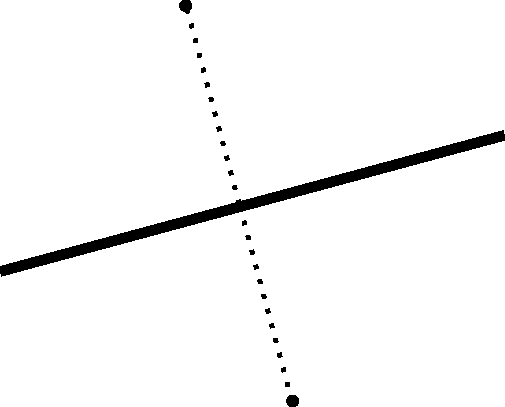
\includegraphics[height=10\baselineskip,keepaspectratio]{figures/equidistant.pdf}
\end{figure}
Let's name this line $L$. From the previous chapter we know how to get the line that's created by the two points $M$ and $N$. If only we knew how to get a perpendicular line over the midpoint of a line segment!

Thankfully that midpoint also satisfies $L$'s equation, $ax+by+c$. The midpoint's coordinates are intuitively:\index{midpoint}

$$ (\frac{x_M + x_N}{2}, \frac{y_M + y_N}{2})$$

Putting them into the equation we can generate a triple of $(a', b', c')$ and then normalize it to get $L$.
\chapter{Normal to a line through a point}
\todo[inline]{Add \emph{Normal to a line through a point}}
\skelpars{2}
\clearpage{}
\myaddthumb{Points and Line Segments}{segments}
\part{Points And Line Segments}
\chapter{Drawing a line segment from its two endpoints}

For any line segment with any slope, \pixels{} must be matched with the infinite
amount of points contained in the segment. As shown in the following figure, a segment \emph{touches} some \pixels{}; we could fill them using an algorithm and get a \bitmap{} of the line segment.

\begin{figure}
\centering
\input{fig2.pdf_tex}
\end{figure}

The algorithm presented here was first derived by Bresenham. In the \emph{Image} implementation, it is used in the \texttt{plot\_line\_width} method.
% From graphic gems vol 1 p 99 (pdf page 124)
\begin{minted}{rust}
pub fn plot_line_width(&mut self, (x1, y1): (i64, i64), (x2, y2): (i64, i64)) {
    /* Bresenham's line algorithm */
    let mut d;
    let mut x: i64;
    let mut y: i64;
    let ax: i64;
    let ay: i64;
    let sx: i64;
    let sy: i64;
    let dx: i64;
    let dy: i64;

    dx = x2 - x1;
    ax = (dx * 2).abs();
    sx = if dx > 0 { 1 } else { -1 };

    dy = y2 - y1;
    ay = (dy * 2).abs();
    sy = if dy > 0 { 1 } else { -1 };

    x = x1;
    y = y1;

    let b = dx / dy;
    let a = 1;
    let double_d = (_wd * f64::sqrt((a * a + b * b) as f64)) as i64;
    let delta = double_d / 2;

    if ax > ay {
        d = ay - ax / 2;
        loop {
            self.plot(x, y);
            if x == x2 {
                return;
            }
            if d >= 0 {
                y = y + sy;
                d = d - ax;
            }
            x = x + sx;
            d = d + ay;
        }
    } else {
        d = ax - ay / 2;
        let delta = double_d / 3;
        loop {
            self.plot(x, y);
            if y == y2 {
                return;
            }
            if d >= 0 {
                x = x + sx;
                d = d - ay;
            }
            y = y + sy;
            d = d + ax;
        }
    }
}
\end{minted}
\todo[inline]{Add some explanation behind the algorithm in \emph{Drawing a line segment from its two endpoints}}
\chapter{Drawing line segments with width}
\begin{minted}{rust}
pub fn plot_line_width(&mut self, (x1, y1): (i64, i64), (x2, y2): (i64, i64), _wd: f64) {
    /* Bresenham's line algorithm */
    let mut d;
    let mut x: i64;
    let mut y: i64;
    let ax: i64;
    let ay: i64;
    let sx: i64;
    let sy: i64;
    let dx: i64;
    let dy: i64;

    dx = x2 - x1;
    ax = (dx * 2).abs();
    sx = if dx > 0 { 1 } else { -1 };

    dy = y2 - y1;
    ay = (dy * 2).abs();
    sy = if dy > 0 { 1 } else { -1 };

    x = x1;
    y = y1;

    let b = dx / dy;
    let a = 1;
    let double_d = (_wd * f64::sqrt((a * a + b * b) as f64)) as i64;
    let delta = double_d / 2;

    if ax > ay {
        d = ay - ax / 2;
        loop {
            self.plot(x, y);
            {
                let total = |_x| _x - (y * dx) / dy + (y1 * dx) / dy - x1;
                let mut _x = x;
                loop {
                    let t = total(_x);
                    if t < -1 * delta || t > delta {
                        break;
                    }
                    _x += 1;
                    self.plot(_x, y);
                }
                let mut _x = x;
                loop {
                    let t = total(_x);
                    if t < -1 * delta || t > delta {
                        break;
                    }
                    _x -= 1;
                    self.plot(_x, y);
                }
            }
            if x == x2 {
                return;
            }
            if d >= 0 {
                y = y + sy;
                d = d - ax;
            }
            x = x + sx;
            d = d + ay;
        }
    } else {
        d = ax - ay / 2;
        let delta = double_d / 3;
        loop {
            self.plot(x, y);
            {
                let total = |_x| _x - (y * dx) / dy + (y1 * dx) / dy - x1;
                let mut _x = x;
                loop {
                    let t = total(_x);
                    if t < -1 * delta || t > delta {
                        break;
                    }
                    _x += 1;
                    self.plot(_x, y);
                }
                let mut _x = x;
                loop {
                    let t = total(_x);
                    if t < -1 * delta || t > delta {
                        break;
                    }
                    _x -= 1;
                    self.plot(_x, y);
                }
            }
            if y == y2 {
                return;
            }
            if d >= 0 {
                x = x + sx;
                d = d - ay;
            }
            y = y + sy;
            d = d + ax;
        }
    }
}
\end{minted}
% Graphics gems vol 1. pdf page 139 "RENDERING FAT LINES ON 2D GRID"

\chapter{Intersection of two line segments}
% Graphics gems vol 2. pdf page 37
Let points $\textbf{1}=(x_1,y_1)$, $\textbf{2} = (x_2, y_2)$, $\textbf{3} = (x_3, y_3)$ and $\textbf{4} = (x_4, y_4)$ and $\textbf{1,2}$, $\textbf{3,4}$ two line segments they form. We wish to find their intersection:

First, get the equation of line $L_{12}$ and line $L_{34}$ from chapter \emph{\nameref{ch:equations-lines}}.

Substitute points $\textbf{3}$ and $\textbf{4}$ in equation $L_{12}$ to compute $r_3 = L_{12}(\textbf{3})$ and $r_4=L_{12}(\textbf{4})$ respectively.

If $r_3 \neq{} 0$, $r_4 \neq{} 0$ and $sgn(r_3)==sign(r_4)$ the line segments don't intersect, so stop.

In $L_{34}$ substitute point $\textbf{1}$ to compute $r_1$, and do the same for point $\textbf{2}$.

If $r_1 \neq{} 0$, $r_2 \neq{} 0$ and $sgn(r_1)==sign(r_2)$ the line segments don't intersect, so stop.

At this point, $L_{12}$ and $L_{34}$ either intersect or are equivalent. Find their intersection point. (Refer to \emph{\nameref{ch:intersection-lines}}.)
\todo[inline]{Add code sample in \emph{Intersection of two line segments}}
\section{\emph{Fast} intersection of two line segments}
% Graphics gems vol 3. pdf page 231
\skelpars{2}
\clearpage{}
\myaddthumb{Points, Lines and Circles}{circles}
\part{Points, Lines and Circles}
\skelpars{2}
\chapter{Equations of a circle}
\todo[inline]{Add \emph{Equations of a circle}}
\skelpars{2}
\chapter{Bounding circle}
% From graphic gems vol 2 pdf page 46
% From Υπολογιστική Γεωμετρία 4.7 page 85 Μικρότατοι περικλείοντες δίσκοι
\attachsource{src/bin/boundingcircle.rs}
\begin{figure}[H]
\centering
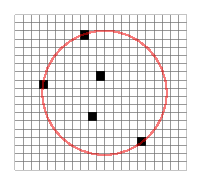
\includegraphics[scale=2,keepaspectratio]{figures/minidisc.pdf}
\end{figure}
A bounding circle is a circle that includes all the points in a given set. Usually we're interested in one of the smallest ones possible.

\begin{figure}[H]
\centering

\includegraphics{figures/minidisc.png}
\end{figure}

We can use the following methodology to find the bounding circle: start from two points and the circle they make up, and for each of the rest of the points check if the circle includes them. If not, make a bounding circle that includes every point up to the current one. To do this, we need some primitive operations.

We will need a way to construct a circle out of two points:\index{circle out of two points}

\begin{figure}[H]
\centering

\includegraphics[scale=0.25,keepaspectratio]{figures/two_points_circle.png}
\end{figure}

\begin{minted}{rust}
  let p1 = points[0];
  let p2 = points[1];
  //The  circle  is  determined  by  two  points,  P  and  Q.  The  center  of the  circle  is
  //at  (P  +  Q)/2.0  and  the  radius  is  |(P  –  Q)/2.0|
  let d_2 = (
  (((p1.0 + p2.0) / 2), (p1.1 + p2.1) / 2),
  (distance_between_two_points(p1, p2) / 2.0),
  );
\end{minted}

And a way to make a circle out of three points:\index{circle out of three points}

\begin{figure}[H]
\centering
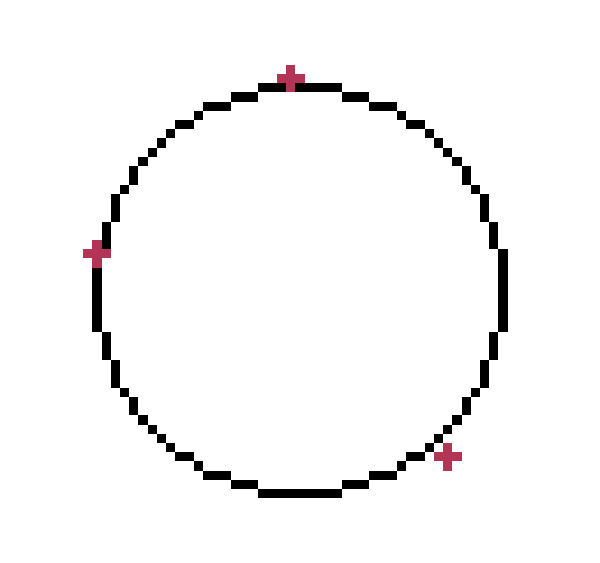
\includegraphics[scale=0.25,keepaspectratio]{figures/triangle_circle.png}
\end{figure}

\begin{minted}{rust}
fn min_circle_w_3_points(q1: Point, q2: Point, q3: Point) -> Circle {
    let (ax, ay) = (q1.0 as f64, q1.1 as f64);
    let (bx, by) = (q2.0 as f64, q2.1 as f64);
    let (cx, cy) = (q3.0 as f64, q3.1 as f64);

    let mut d = 2. * (ax * (by - cy) + bx * (cy - ay) + cx * (ay - by));
    if d == 0.0 {
        d = std::cmp::max(
            std::cmp::max(
                distance_between_two_points(q1, q2) as i64,
                distance_between_two_points(q2, q3) as i64,
            ),
            distance_between_two_points(q1, q3) as i64,
        ) as f64
            / 2.;
    }
    let ux = ((ax * ax + ay * ay) * (by - cy)
        + (bx * bx + by * by) * (cy - ay)
        + (cx * cx + cy * cy) * (ay - by))
        / d;
    let uy = ((ax * ax + ay * ay) * (cx - bx)
        + (bx * bx + by * by) * (ax - cx)
        + (cx * cx + cy * cy) * (bx - ax))
        / d;
    let mut center = (ux as i64, uy as i64);

    if center.0 < 0 {
        center.0 = 0;
    }
    if center.1 < 0 {
        center.1 = 0;
    }
    let d = distance_between_two_points(center, q1);
    (center, d)
}
\end{minted}

The algorithm:

\begin{minted}{rust}
use bitmappers_companion::*;
use minifb::{Key, Window, WindowOptions};
use rand::seq::SliceRandom;
use rand::thread_rng;
use std::f64::consts::{FRAC_PI_2, PI};

include!("../me.xbm.rs");

const WINDOW_WIDTH: usize = 400;
const WINDOW_HEIGHT: usize = 400;

pub fn distance_between_two_points(p_k: Point, p_l: Point) -> f64 {
    let (x_k, y_k) = p_k;
    let (x_l, y_l) = p_l;
    let xlk = x_l - x_k;
    let ylk = y_l - y_k;
    f64::sqrt((xlk * xlk + ylk * ylk) as f64)
}

fn image_to_points(image: &Image) -> Vec<Point> {
    let mut ret = Vec::with_capacity(image.bytes.len());
    for y in 0..(image.height as i64) {
        for x in 0..(image.width as i64) {
            if image.get(x, y) == Some(BLACK) {
                ret.push((x, y));
            }
        }
    }
    ret
}

type Circle = (Point, f64);

fn bc(image: &Image) -> Circle {
    let mut points = image_to_points(image);
    points.shuffle(&mut thread_rng());
    min_circle(&points)
}
fn min_circle(points: &[Point]) -> Circle {
    let mut points = points.to_vec();
    points.shuffle(&mut thread_rng());

    let p1 = points[0];
    let p2 = points[1];
    //The  circle  is  determined  by  two  points,  P  and  Q.  The  center  of the  circle  is
    //at  (P  +  Q)/2.0  and  the  radius  is  |(P  –  Q)/2.0|
    let d_2 = (
        (((p1.0 + p2.0) / 2), (p1.1 + p2.1) / 2),
        (distance_between_two_points(p1, p2) / 2.0),
    );

    let mut d_prev = d_2;

    for i in 2..points.len() {
        let p_i = points[i];
        if distance_between_two_points(p_i, d_prev.0) <= (d_prev.1) {
            // then d_i = d_(i-1)
        } else {
            let new = min_circle_w_point(&points[..i], p_i);
            if distance_between_two_points(p_i, new.0) <= (new.1) {
                d_prev = new;
            }
        }
    }

    d_prev
}

fn min_circle_w_point(points: &[Point], q: Point) -> Circle {
    let mut points = points.to_vec();

    points.shuffle(&mut thread_rng());
    let p1 = points[0];
    //The  circle  is  determined  by  two  points,  P_1  and  Q.  The  center  of the  circle  is
    //at  (P_1  +  Q)/2.0  and  the  radius  is  |(P_1  –  Q)/2.0|
    let d_1 = (
        (((p1.0 + q.0) / 2), (p1.1 + q.1) / 2),
        (distance_between_two_points(p1, q) / 2.0),
    );

    let mut d_prev = d_1;

    for j in 1..points.len() {
        let p_j = points[j];
        if distance_between_two_points(p_j, d_prev.0) <= (d_prev.1) {
            //d_prev = d_prev;
        } else {
            let new = min_circle_w_points(&points[..j], p_j, q);
            if distance_between_two_points(p_j, new.0) <= (new.1) {
                d_prev = new;
            }
        }
    }
    d_prev
}

fn min_circle_w_points(points: &[Point], q1: Point, q2: Point) -> Circle {
    let mut points = points.to_vec();

    let d_0 = (
        (((q1.0 + q2.0) / 2), (q1.1 + q2.1) / 2),
        (distance_between_two_points(q1, q2) / 2.0),
    );

    let mut d_prev = d_0;
    for k in 0..points.len() {
        let p_k = points[k];
        if distance_between_two_points(p_k, d_prev.0) <= (d_prev.1) {
        } else {
            let new = min_circle_w_3_points(q1, q2, p_k);
            if distance_between_two_points(p_k, new.0) <= (new.1) {
                d_prev = new;
            }
        }
    }
    d_prev
}

fn min_circle_w_3_points(q1: Point, q2: Point, q3: Point) -> Circle {
    let (ax, ay) = (q1.0 as f64, q1.1 as f64);
    let (bx, by) = (q2.0 as f64, q2.1 as f64);
    let (cx, cy) = (q3.0 as f64, q3.1 as f64);

    let mut d = 2. * (ax * (by - cy) + bx * (cy - ay) + cx * (ay - by));
    if d == 0.0 {
        d = std::cmp::max(
            std::cmp::max(
                distance_between_two_points(q1, q2) as i64,
                distance_between_two_points(q2, q3) as i64,
            ),
            distance_between_two_points(q1, q3) as i64,
        ) as f64
            / 2.;
    }
    let ux = ((ax * ax + ay * ay) * (by - cy)
        + (bx * bx + by * by) * (cy - ay)
        + (cx * cx + cy * cy) * (ay - by))
        / d;
    let uy = ((ax * ax + ay * ay) * (cx - bx)
        + (bx * bx + by * by) * (ax - cx)
        + (cx * cx + cy * cy) * (bx - ax))
        / d;
    let mut center = (ux as i64, uy as i64);

    if center.0 < 0 {
        center.0 = 0;
    }
    if center.1 < 0 {
        center.1 = 0;
    }
    let d = distance_between_two_points(center, q1);
    (center, d)
}

fn main() {
    let mut buffer: Vec<u32> = vec![WHITE; WINDOW_WIDTH * WINDOW_HEIGHT];
    let mut window = Window::new(
        "Test - ESC to exit",
        WINDOW_WIDTH,
        WINDOW_HEIGHT,
        WindowOptions {
            title: true,
            //borderless: true,
            resize: true,
            //transparency: true,
            ..WindowOptions::default()
        },
    )
    .unwrap();

    // Limit to max ~60 fps update rate
    window.limit_update_rate(Some(std::time::Duration::from_micros(16600)));

    let mut full = Image::new(WINDOW_WIDTH, WINDOW_HEIGHT, 0, 0);
    let mut image = Image::new(ME_WIDTH, ME_HEIGHT, 45, 45);
    image.bytes = bits_to_bytes(ME_BITS, ME_WIDTH);
    let (center, r) = bc(&image);
    image.draw_outline();

    full.plot_circle((center.0 + 45, center.1 + 45), r as i64, 0.);
    while window.is_open() && !window.is_key_down(Key::Escape) && !window.is_key_down(Key::Q) {
        image.draw(&mut buffer, BLACK, None, WINDOW_WIDTH);
        full.draw(&mut buffer, BLACK, None, WINDOW_WIDTH);

        window
            .update_with_buffer(&buffer, WINDOW_WIDTH, WINDOW_HEIGHT)
            .unwrap();

        let millis = std::time::Duration::from_millis(100);

        std::thread::sleep(millis);
    }
}
\end{minted}
\clearpage{}
\myaddthumb{Curves other than circles}{curves}
\part{Curves other than circles}
\chapter{Parametric elliptical arcs}
\todo[inline]{Add \emph{Parametric elliptical arcs}}
% Graphics gems vol 3. pdf page 196
\skelpars{2}
\clearpage{}
\myaddthumb{Points, Lines and Shapes}{shapes}
\part{Points, Lines and Shapes}
%\chapter{Triangles}
%\section{Making a triangle from a point and given angles}
%\chapter{Rectangles, parallelograms}
\chapter{Union, intersection and difference of polygons}
\todo[inline]{Add \emph{Union, intersection and difference of polygons}}
% Graphics gems vol 2. pdf page 63
\skelpars{2}

\chapter{Centroid of polygon}\index{centroid}
\todo[inline]{Add \emph{Centroid of polygon}}
% Graphics gems vol 4. pdf page 14
\skelpars{2}
\chapter{Flood filling}
\todo[inline]{Add \emph{Flood filling}}
\skelpars{2}
% Graphics gems vol 1. pdf page 296 "SEED FILL"
% Graphics gems vol 1. pdf page 299 "FILLING A REGION IN A FRAMEBUFFER"
\clearpage{}
\myaddthumb{Vectors, matrices and transformations}{trans\-for\-ma\-tions}
\part{Vectors, matrices and trans\-for\-ma\-tions}
\chapter{Rotation of a \bitmap{}}

\[
  p' =
  \begin{bmatrix}
    cosθ & -sinθ\\
    sinθ & cosθ
  \end{bmatrix}
  \begin{bmatrix}
    x_{p}\\
    y_{p}
  \end{bmatrix}
\]

\begin{equation*}
  c = cosθ,\\\\
  s = sinθ,\\
  x_{p'} = x_{p}c-y_{p}s,\\
  y_{p'} = x_{p}s+y_{p}c.
\end{equation*}

Let's load an \texttt{xface}. We will use \texttt{bits\_to\_bytes} (See Introduction).
%
\attachsource{src/bin/rotation.rs}%
%
%
\begin{minted}{rust}
include!("dmr.rs");

const WINDOW_WIDTH: usize = 100;
const WINDOW_HEIGHT: usize = 100;

let mut image = Image::new(DMR_WIDTH, DMR_HEIGHT, 25, 25);
image.bytes = bits_to_bytes(DMR_BITS, DMR_WIDTH);
\end{minted}

\begin{figure}[H]
\centering
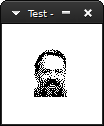
\includegraphics{figures/ch11-1.png}
\end{figure}

This is the \texttt{xface} of \texttt{dmr}. Instead of displaying the \bitmap{}, this time we will rotate it $0.5$ radians. Setup our image first:


\begin{minted}{rust}
let mut image = Image::new(DMR_WIDTH, DMR_HEIGHT, 25, 25);
image.draw_outline();
let dmr = bits_to_bytes(DMR_BITS, DMR_WIDTH);
\end{minted}

And then, loop for each byte in \texttt{dmr}'s face and apply the rotation transformation.

\begin{minted}{rust}
let angle = 0.5;

let c = f64::cos(angle);
let s = f64::sin(angle);

for y in 0..DMR_HEIGHT {
    for x in 0..DMR_WIDTH {
        if dmr[y * DMR_WIDTH + x] == BLACK {
            let x = x as f64;
            let y = y as f64;
            let xr = x * c - y * s;
            let yr = x * s + y * c;
            image.plot(xr as i64, yr as i64);
        }
    }
}
\end{minted}

The result:

\begin{figure}[H]
\centering
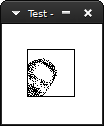
\includegraphics{figures/ch11-2.png}
\end{figure}

We didn't mention in the beginning that the rotation has to be relative to a \emph{point} and the given transformation is relative to the \emph{origin}, in this case the upper left corner $(0,0)$. So \texttt{dmr} was rotated relative to the origin\,:
\begin{figure}
\centering
  \def\svgscale{0.6}
\input{cartesian_grid_dmr_1.pdf_tex}
  \def\svgscale{0.6}
\input{cartesian_grid_dmr_2.pdf_tex}
\end{figure}

{\centering{}
\noindent(the distance to the origin (actually 0 \pixels{}) has been exaggerated for the sake of the example)
}

Usually, we want to rotate something relative to itself. The right point to choose is the \emph{centroid} of the object.\index{centroid}

If we have a list of $n$ points, the centroid is calculated as:

$$ x_c = \frac{1}{n}\sum_{i=0}^{n} x_i $$
$$ y_c = \frac{1}{n}\sum_{i=0}^{n} y_i $$

Since in this case we have a rectangle, the centroid has coordinates of half the width and half the height.

By subtracting the centroid from each point before we apply the transformation and then adding it back after we get what we want:

Here's it visually: First subtract the center point.

\begin{figure}
\centering
\def\svgscale{0.6}
\input{cartesian_grid_dmr_3.pdf_tex}
\end{figure}

Then, rotate.

\begin{figure}
\centering
\def\svgscale{0.6}
\input{cartesian_grid_dmr_4.pdf_tex}
\end{figure}

And subtract back to the original position.

\begin{figure}
\centering
\def\svgscale{0.6}
\input{cartesian_grid_dmr_5.pdf_tex}
\end{figure}

In code:

\begin{minted}{rust}
let center_point = ((DMR_WIDTH/2) as i64, (DMR_HEIGHT/2) as i64);
for y in 0..DMR_HEIGHT {
    for x in 0..DMR_WIDTH {
        if dmr[y * DMR_WIDTH + x] == BLACK {
            let x = (x as i64 -center_point.0) as f64;
            let y = (y as i64 -center_point.1) as f64;
            let xr = x * c - y * s;
            let yr = x * s + y * c;
            image.plot(xr as i64+center_point.0,
                       yr as i64 + center_point.1);
        }
    }
}
\end{minted}

The result: 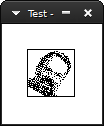
\includegraphics{figures/ch11-3.png}

\section{Fast 2D Rotation}
\todo[inline]{Add \emph{Fast 2D Rotation}}
% Graphics gems vol 1. pdf page 456 
\skelpars{2}
\chapter{90\textdegree{} Rotation of a \bitmap{} by parallel recursive subdivision}
\todo[inline]{Add \emph{90\textdegree{} Rotation of a \bitmap{} by parallel recursive subdivision}}
% Graphics gems vol 2. pdf page 113 
\skelpars{2}
\chapter{Magnification/Scaling}
\begin{figure}[H]
\centering
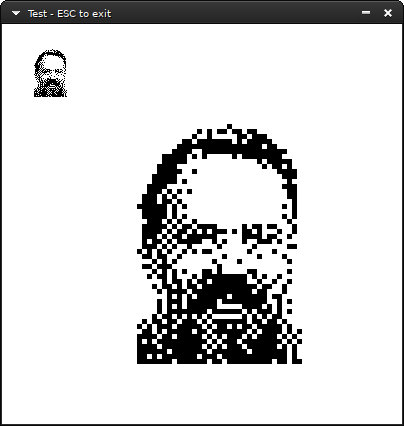
\includegraphics{figures/scaled_dmr.png}
\end{figure}

\attachsource{src/bin/scale.rs}%
\begin{minted}{rust}
let mut original = Image::new(DMR_WIDTH, DMR_HEIGHT, 25, 25);
original.bytes = bits_to_bytes(DMR_BITS, DMR_WIDTH);
original.draw(&mut buffer, BLACK, None, WINDOW_WIDTH);

let mut scaled = Image::new(DMR_WIDTH * 5, DMR_HEIGHT * 5, 100, 100);
let mut sx: i64; //source
let mut sy: i64; //source
let mut dx: i64; //destination
let mut dy: i64 = 0; //destination

let og_height = original.height as i64;
let og_width = original.width as i64;
let scaled_height = scaled.height as i64;
let scaled_width = scaled.width as i64;

while dy < scaled_height {
    sy = (dy * og_height) / scaled_height;
    dx = 0;
    while dx < scaled_width {
        sx = (dx * og_width) / scaled_width;
        if original.get(sx, sy) == Some(BLACK) {
            scaled.plot(dx, dy);
        }
        dx += 1;
    }
    dy += 1;
}
scaled.draw(&mut buffer, BLACK, None, WINDOW_WIDTH);
\end{minted}
\section{Smoothing enlarged \bitmaps{}}
\todo[inline]{Add \emph{Smoothing enlarged \bitmaps{}}}
% https://en.wikipedia.org/wiki/Hqx
% Graphics gems vol 1. pdf page 189 "SMOOTHING ENLARGED MONOCHROME IMAGES"
\skelpars{2}
\section{Stretching lines of \bitmaps{}}
\todo[inline]{Add \emph{Stretching lines of \bitmaps{}}}
% Graphics gems vol 3. pdf page 34 "FAST BITMAP STRETCHING"
\skelpars{2}
\chapter{Mirroring}
\todo[inline]{Add screenshots and figure and code in \emph{Mirroring}}
Mirroring to an axis is the transformation of one coordinate to its equidistant value across the axis:

To mirror a \pixel across the $x$ axis, simply multiply its coordinates with the following matrix:

\[
  M_x =
  \begin{bmatrix}
    1 & 0\\
    0 & -1
  \end{bmatrix}
\]

This results in the $y$ coordinate's sign being flipped.

For $y$-mirroring, the transformation follows the same logic:

\[
  M_y =
  \begin{bmatrix}
    -1 & 0\\
    0 & 1
  \end{bmatrix}
\]

% Geometric tools for computer graphics  pdf page 195, "Reflection"
\chapter{Shearing}
\attachsource{src/bin/shearing.rs}%
Simple shearing\index{shearing} is the transformation of one dimension by a distance proportional to the other dimension, In $x$-shearing (or horizontal shearing) only the $x$ coordinate is affected, and likewise in $y$-shearing only $y$ as well.

% Geometric tools for computer graphics  pdf page 200, "Shearing"
\begin{figure}[H]
\centering
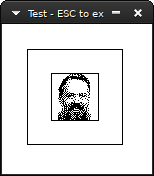
\includegraphics{figures/shearing-0.png}
\end{figure}

With $l$ being equal to the desired tilt away from the $y$ axis, the transformation is described by the following matrix:

\[
  S_x =
  \begin{bmatrix}
    1 & l\\
    0 & 1
  \end{bmatrix}
\]

Which is as simple as this function:

\begin{minted}{rust}
fn shear_x((x_p, y_p): (i64, i64), l: f64) -> (i64, i64) {
    (x_p+(l*(y_p as f64)) as i64, y_p)
}
\end{minted}

\begin{figure}[H]
\centering
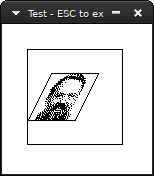
\includegraphics{figures/shearing-1.png}
\end{figure}

For $y$-shearing, we have the following:

\[
  S_y =
  \begin{bmatrix}
    1 & 0\\
    l & 1
  \end{bmatrix}
\]

\begin{minted}{rust}
fn shear_y((x_p, y_p): (i64, i64), l: f64) -> (i64, i64) {
    (x_p, (l*(x_p as f64)) as i64 + y_p)
}
\end{minted}

\begin{figure}[H]
\centering
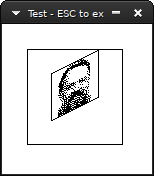
\includegraphics{figures/shearing-2.png}
\end{figure}

A full example:
\begin{minted}{rust}
include!("../dmr.xbm.rs");

const WINDOW_WIDTH: usize = 200;
const WINDOW_HEIGHT: usize = 200;

fn shear_x((x_p, y_p): (i64, i64), l: f64) -> (i64, i64) {
    (x_p+(l*(y_p as f64)) as i64, y_p)
}
fn shear_y((x_p, y_p): (i64, i64), l: f64) -> (i64, i64) {
    (x_p, (l*(x_p as f64)) as i64 + y_p)
}

let mut image = Image::new(DMR_WIDTH, DMR_HEIGHT, 25, 25);
image.bytes = bits_to_bytes(DMR_BITS, DMR_WIDTH);
image.draw_outline();

let l = -0.5;
let mut sheared = Image::new(DMR_WIDTH*2, DMR_HEIGHT*2, 25, 25);
for x in 0..DMR_WIDTH {
    for y in 0..DMR_HEIGHT  {
        if image.bytes[y * DMR_WIDTH + x] == BLACK {
          let p = shear_x((x as i64 ,y as i64 ), l);
          sheared.plot(p.0+(DMR_WIDTH/2) as i64, p.1+(DMR_HEIGHT/2) as i64); 
        }
    }
}
sheared.draw_outline();
\end{minted}
\section{The relationship between shearing factor and angle}
\begin{figure}[H]
\centering

\includegraphics[width=\textwidth,keepaspectratio]{figures/xshear.pdf}
\end{figure}
Shearing is a delta movement in one dimension, thus the point before moving and the point after form an angle with the $x$ axis. To move a point $(x, 0)$ by 30\textdegree{} forward we will have the new point $(x+f, 0)$ where $f$ is the shear factor. These two points and $(x, h)$ where $h$ is the height of the \bitmap{} form a triangle, thus the following are true:

$$cot\theta{} = \frac{h}{f}$$

Therefore to find your factor for any angle $\theta{}$ replace its cotangent in the following formula:

$$f = \frac{h}{cot\theta{}}$$

For example to shear by $-$30\textdegree{} (meaning the \bitmap{} will move to the right, since rotations are always clockwise) we need $cot(-30deg) = -\sqrt{3}$ and $f=-\frac{h}{\sqrt{3}}$.

\chapter{Projections}
\todo[inline]{Add \emph{Projections}}
% Geometric tools for computer graphics  pdf page 205, "Projections"
\skelpars{2}
\clearpage{}
\myaddthumb{Addendum}{ad\-den\-dum}
\part{Addendum}
\section{Faster Drawing a line segment from its two endpoints using Symmetry}
\todo[inline]{Add \emph{Faster Drawing a line segment from its two endpoints using Symmetry}}
% From graphic gems vol 1 p 103 (pdf page 128)
\skelpars{2}

\chapter{Joining the ends of two wide line segments together}
\todo[inline]{Add \emph{Joining the ends of two wide line segments together}}
% Graphics gems vol 1. pdf page 132 "AN ALGORITHM FOR FILLING IN 2D WIDE LINE BEVEL JOINTS"
\skelpars{2}
\chapter{Composing monochrome \bitmaps{} with separate alpha channel data}
\todo[inline]{Add \emph{Composing monochrome \bitmaps{} with separate alpha channel data}}
% Graphics gems vol 3. pdf page 64 "COMPOSING BW BITMAPS
\skelpars{2}
\chapter{Orthogonal connection of two points}
\todo[inline]{Add \emph{Orthogonal connection of two points}}
% Graphics gems vol 3. pdf page 205 "SIMPLE CONNECTION ALGORITHM FOR 2D DRAWING"
\skelpars{2}
\chapter{Join segments with round corners}
\todo[inline]{Add \emph{Join segments with round corners}}
% Graphics gems vol 3. pdf page 225 "JOINING TWO LINES WITH A CIRCULAR ARC FILLET"
\skelpars{2}
\chapter{Faster line clipping}
\todo[inline]{Add \emph{Faster line clipping}}
% Graphics gems vol 5. pdf page 323 "FASTER PIXEL PERFECT LINE CLIPPING"
\skelpars{2}
\chapter{Space-filling Curves}
\todo[inline]{Add \emph{Space-filling Curves}}
% Graphics gems vol 2. pdf page 58
\skelpars{1}
\clearpage{}
\section{Hilbert curves}
\todo[inline]{Add \emph{Hilbert curves} explanation}
\begin{figure}[H]
\centering
  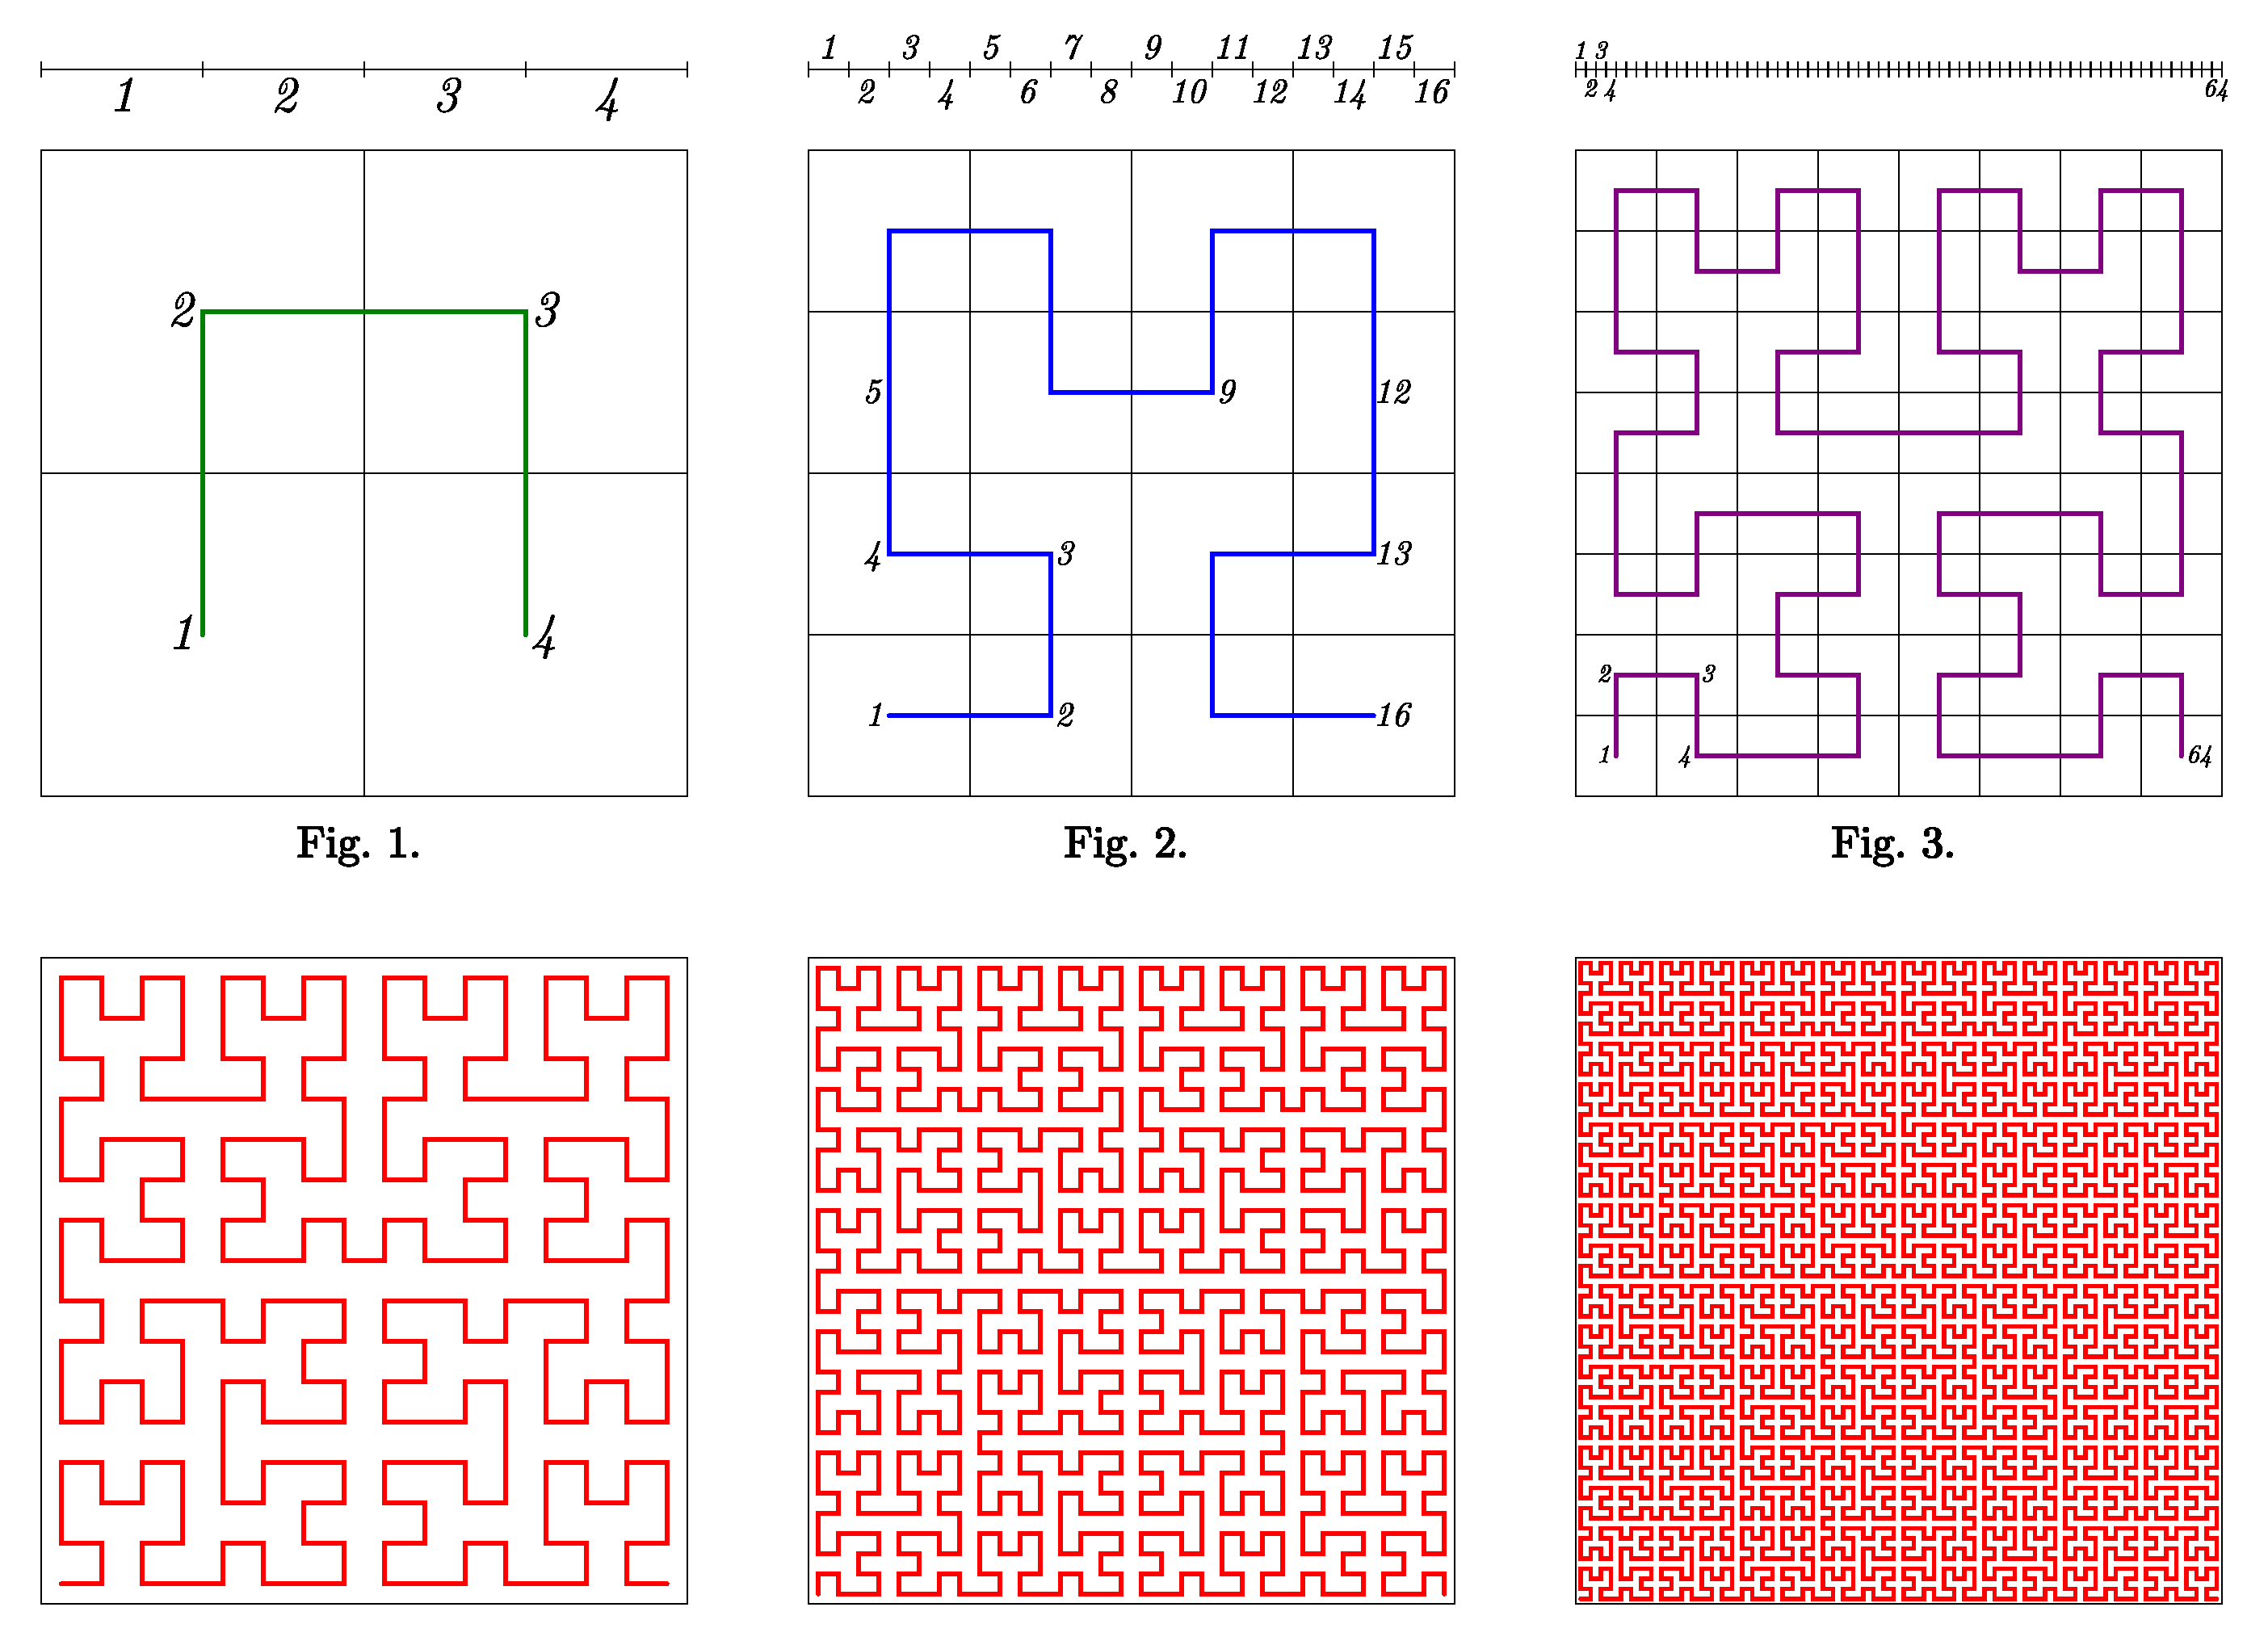
\includegraphics[height=15\baselineskip,keepaspectratio]{figures/HilbertCurve.pdf}\par
  {\scriptsize{}The first six iterations of the Hilbert curve \myurl{https://commons.wikimedia.org/wiki/File:Hilbert\_curve.svg}{by \texttt{Braindrain0000}}}
\end{figure}
\attachsource{src/bin/hilbert.rs}
Here's a simple algorithm for drawing a Hilbert curve.\footnote{Griffiths, J. G. (1985). \emph{Table-driven algorithms for generating space-filling curves}. Computer-Aided Design, 17(1), 37–41. \texttt{doi:10.1016/0010-4485(85)90009-0}}
\begin{minted}{rust}
const HILBERT: &[&[usize]] = &[
    &[22, 10, 16, 38],
    &[10, 22, 24, 48],
    &[44, 36, 30, 18],
    &[36, 44, 42, 28],
];

fn curve(img: &mut Image, k: usize, order: i64, mut x: i64, mut y: i64) -> (i64, i64) {
    const STEP_SIZE: i64 = 5;
    let mut row: usize;
    let mut direction: usize;
    if order > 0 {
        for j in 0..4 {
            let step = HILBERT[k][j];
            row = (step / 10) - 1;
            let (xn, yn) = curve(img, row, order - 1, x, y);
            x = xn;
            y = yn;
            direction = step % 10;
            let prev = (x, y);
            match direction {
                8 => {
                    // null op
                }
                2 => {
                    //N
                    y -= STEP_SIZE;
                }
                1 => {
                    // NE
                    y -= STEP_SIZE;
                    x += STEP_SIZE;
                }
                0 => {
                    //E
                    x += STEP_SIZE;
                }
                7 => {
                    //SE
                    x += STEP_SIZE;
                    y += STEP_SIZE;
                }
                6 => {
                    //S
                    y += STEP_SIZE;
                }
                5 => {
                    //SW
                    y += STEP_SIZE;
                    x -= STEP_SIZE;
                }
                4 => {
                    //W
                    x -= STEP_SIZE;
                }
                3 => {
                    //NW
                    y -= STEP_SIZE;
                    x -= STEP_SIZE;
                }
                other => unreachable!("{}", other),
            }
            img.plot_line_width(prev, (x, y), 0.);
        }
    }
    (x, y)
}
\end{minted}
\begin{minted}{rust}
let mut image = Image::new(WINDOW_WIDTH, WINDOW_WIDTH, 0, 0);
curve(&mut image, 0, 7, 0, WINDOW_WIDTH as i64);
\end{minted}
\begin{figure}
\centering
  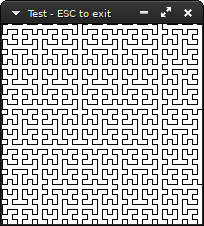
\includegraphics[keepaspectratio,scale=1]{figures/hilbert.png}
\end{figure}
\section{Sierpinshi curve}
\begin{figure}
  \centering
  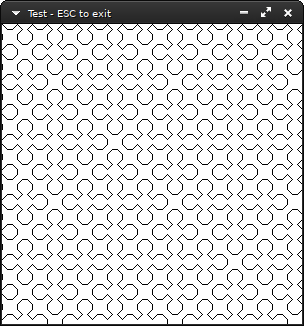
\includegraphics[keepaspectratio,scale=1]{figures/sierpinshi.png}
\end{figure}

Switching the table from the Hilbert implementation to this:

\begin{minted}{rust}
const SIERP: &[&[usize]] = &[
    &[17, 25, 33, 41],
    &[17, 20, 41, 18],
    &[25, 36, 17, 28],
    &[33, 44, 25, 38],
    &[41, 12, 33, 48],
];
\end{minted}
And switching two lines from the function to
\begin{minted}{diff}
 - let step = HILBERT[k][j];
 - row = (step / 10) - 1;
 + let step = SIERP[k][j];
 + row = (step / 10);
\end{minted}
You can draw a Sierpinshi curve of order $n$ by calling \texttt{curve(\&mut image, 0,n+1, 0, 0)}.
\section{Peano curves}
\todo[inline]{Add \emph{Peano curves}}
\skelpars{1}
\section{Z-order curves}
\todo[inline]{Add \emph{Z-order curves}}
\skelpars{1}
\clearpage{}
\stopthumb
\backmatter
\bookmarksetup{startatroot}
\cleardoublepage
\printindex
\cleardoublepage
\bookmarksetup{startatroot}
\colophontitle{About this text}
\pdfbookmark{About this text}{colophon}
\thispagestyle{empty}
\colophontitlesize{25pt}
\begin{colophon}
\noindent{}The text has been typeset in {\cm{}\XeLaTeX{}} using the \texttt{book} class and:
\begin{itemize}
  \item \textbf{Redaction} for the main text.
  \item \textbf{\fira{}Fira Sans} for referring to the programming language \Rust{}\,.
  \item \textbf{\pixelfont{}Redaction20} for referring to the words \bitmap{} and \pixels{} as a concept.
\end{itemize}
\end{colophon}
\clearpage{}
\listoftodos{}
\end{document}
